\documentclass[11pt]{article}
\usepackage[paperwidth=8.5in, paperheight=11in]{geometry}

\usepackage{../tjimo}

% \def\solution{\comment}

\newcommand{\sevenpoints}{Time limit: 30 minutes.}
\newcommand{\righthead}{\fdbox{Round}{Practice Power}}

\begin{document}

Unlike the other rounds, just getting the answer right is not enough on the Power Round. Make sure you explain your answer and use words
to describe how you arrived at your answer. In the words of middle school math teachers across the nation -- no work, no credit!

Problems are meant to lead into each other. You may use results from previous problems to help you on later problems!

\section{What is a Graph?}

You might have heard of a graph in your math class as a plot with an $x$ and $y$ axis. Or maybe in science you looked at
bar graphs and pie graphs. Maybe in history you took a look at line graphs. But the graphs we are going to talk about today
are none of the above.

\subsection{Some Introduction}

At its core, a \textit{graph} consists of two sets: a group of objects, and a group of connectors that each join two objects.

To gain insight into what a graph is, let's first consider flights that connect airports around the world.
We depend on airplanes to travel quickly and efficiently. When we want to travel between major cities,
like between D.C. and Boston, we can often take a single flight to make the trip. Enough people want to travel between
these two cities for it to be economical to offer a single flight between them.

However, it is not always the case that single-flight trips are economically feasible, either due to lack of demand
or due to needing to refuel. To travel from London to Yellowstone, for example, one must first stop in Atlanta, hop
on a connecting flight to Denver, and then finally travel to Yellowstone. Denver and Atlanta are what we call
hubs, since they are very large airports that accommodate heavy travel loads. To travel between smaller airports, we often
need to stop at one of these larger hubs.

\begin{center}
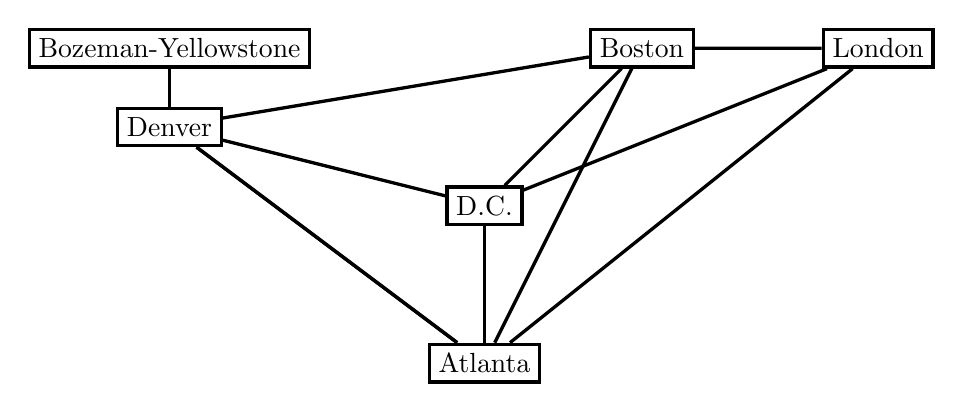
\begin{tikzpicture}[very thick,level/.style={sibling distance=70mm/#1}]
\draw (0, 0) node[draw, shape=rectangle] (a) {D.C.};
\draw (-4, 1) node[draw, shape=rectangle] (b) {Denver};
\draw (0, -2) node[draw, shape=rectangle] (c) {Atlanta};
\draw (2, 2) node[draw, shape=rectangle] (d) {Boston};
\draw (5, 2) node[draw, shape=rectangle] (e) {London};
\draw (-4, 2) node[draw, shape=rectangle] (f) {Bozeman-Yellowstone};
\draw (a) -- (b) -- (c) -- (d) -- (e);
\draw (b) -- (f);
\draw (c) -- (b);
\draw (a) -- (d);
\draw (b) -- (d);
\draw (a) -- (c);
\draw (c) -- (e);
\draw (a) -- (e);
\end{tikzpicture}
\end{center}

Our connections between our cities in the graph represent only direct connections between
cities, but from our diagram, we can still see it is possible to travel between any two
cities in our graph.

Neither the exact position of each city nor how connections might intersect 
matters. In other words, the way we draw a graph on paper does not change its properties, and for the most part
is not useful to us. The following is an equivalent graph:

\begin{center}
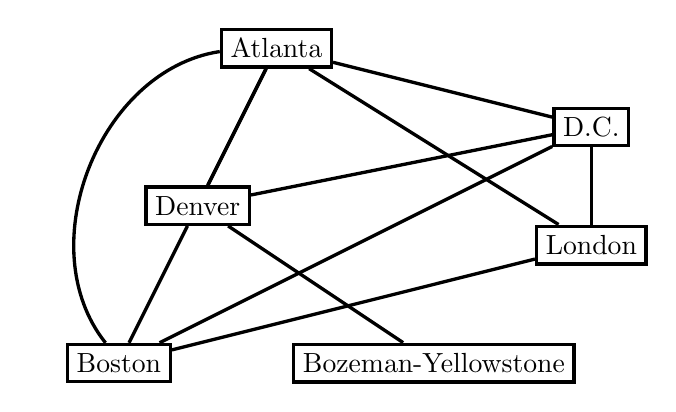
\begin{tikzpicture}[very thick,level/.style={sibling distance=70mm/#1}]
\draw (5, 3) node[draw, shape=rectangle] (a) {D.C.};
\draw (0, 2) node[draw, shape=rectangle] (b) {Denver};
\draw (1, 4) node[draw, shape=rectangle] (c) {Atlanta};
\draw (-1, 0) node[draw, shape=rectangle] (d) {Boston};
\draw (5, 1.5) node[draw, shape=rectangle] (e) {London};
\draw (3, 0) node[draw, shape=rectangle] (f) {Bozeman-Yellowstone};
\draw (a) -- (b) -- (c);
\path (c) edge [bend right=60] (d);
\draw (d) -- (e);
\draw (b) -- (f);
\draw (c) -- (b);
\draw (a) -- (d);
\draw (b) -- (d);
\draw (a) -- (c);
\draw (c) -- (e);
\draw (a) -- (e);
\end{tikzpicture}
\end{center}

The only characteristics of a graph we care about are the objects (in this case, cities) themselves, which we'll call \textit{vertices},
and the connections joining the objects, which we'll call \textit{edges}.

\subsection{Definition of a Graph}

We now have the background necessary to present the mathematical definition of a graph:

\begin{definition}
\label{def:graph}
A \textit{graph} $G(V,E)$ consists of a set of vertices $V$ and a set of edges $E$. 

\begin{center}
\begin{tikzpicture}[very thick,level/.style={sibling distance=70mm/#1}]
\draw (0, 0) node [vertex] (a) {$a$};
\draw (2, 1) node [vertex] (b) {$b$};
\draw (2, -1) node  [vertex] (c) {$c$};
\draw (4, 0) node [vertex] (d) {$d$};
\draw (a) -- (b);
\draw (b) -- (c);
\draw (c) -- (d);
\draw (b) -- (d);
\draw (a) -- (c);
\draw (6, -1) node [vertex] (e) {$e$};
\draw (6, 1) node [vertex] (f) {$f$};
\draw (8, 1) node [vertex] (g) {$g$};
\draw (8, -1) node [vertex] (h) {$h$};
\draw (e) -- (f) -- (g) -- (h) -- (f);
\draw (10, 0) node[vertex] (i) {$i$};
\draw (12, 0) node[vertex] (j) {$j$};
\draw (i) -- (j);
\end{tikzpicture}
\end{center}
\end{definition}

\begin{definition}
\label{def:edge}
An \textit{edge} is a collection of exactly two vertices. In the above graph, there is an edge
between $a$ and $b$, so $\{a, b\}$ is an edge. Note that $\{a,b\}$ is the same edge as $\{b,a\}$.
\end{definition}

\begin{definition}
\label{def:set}
A \textit{set} is a collection of any number of objects. In the above graph, we have the set of vertices
\[V=\{a, b, c, d, e, f, g, h, i, j\}.\]
We also have the set of edges
\[E=\{\{a,b\}, \{b,c\}, \{c,d\},\{b,d\},\{a,c\},\{e,f\},\{f,g\},\{g,h\},\{h,f\},\{i,j\} \}.\]
\end{definition}

\begin{definition}
\label{def:cardinality}
Given a set $A$, the cardinality $\abs{A}$ denotes the number of elements in $A$.
\end{definition}

\begin{problem}[1 point] % problem 1
Evaluate $\abs{V}$ and $\abs{E}$ for the sets $V$ and $E$ in Definition \ref{def:set}, the definition of the set.
Note that $\{a,b\}$ counts as one single edge.
\end{problem}

\begin{solution}
Answer: $\abs{V} = \abs{E} = \boxed{10}$. \\
There are 10 vertices and 10 edges in the graph.
\end{solution}

\begin{problem}[1 point] % 2
Draw any graph with 5 vertices and 8 edges.
\end{problem}

\begin{solution}
The following graph has 5 vertices and 8 edges.
\begin{center}
\begin{tikzpicture}[very thick,level/.style={sibling distance=70mm/#1}]
\draw (6, -1) node [vertex] (a) {$a$};
\draw (6, 1) node [vertex] (b) {$b$};
\draw (8, 1) node [vertex] (c) {$c$};
\draw (8, -1) node [vertex] (d) {$d$};
\draw (10, 0) node [vertex] (e) {$e$};
\draw (a) -- (b) -- (c) -- (d) -- (a) -- (c) -- (e) -- (d) -- (b);
\end{tikzpicture}
\end{center}
\end{solution}

\subsection{Graph Basics}

\begin{definition}
\label{def:degree}
The $degree$ of a vertex is the number of edges that connect that vertex to another. For vertex $b$ in the following graph, we write $deg(b) = 3$,
meaning the degree of $b$ is 3.
\begin{center}
\begin{tikzpicture}[very thick,level/.style={sibling distance=70mm/#1}]
\draw (0, 0) node [vertex] (a) {$a$};
\draw (2, 1) node [vertex] (b) {$b$};
\draw (2, -1) node  [vertex] (c) {$c$};
\draw (4, 0) node [vertex] (d) {$d$};
\draw (a) -- (b);
\draw (b) -- (c);
\draw (c) -- (d);
\draw (b) -- (d);
\draw (a) -- (c);
\end{tikzpicture}
\end{center}
\end{definition}

\begin{problem}[3 points] % 3
Show that the total number of edges in a graph is equal to
\[\frac{1}{2} \cdot \sum_{\text{all vertices $v$}} deg(v).\]
The symbol $\sum$ means add up $deg(v)$ over all vertices $v$. In the graph in Definition \ref{def:degree},
\begin{align*}
\sum_{\text{all vertices $v$}} deg(v) &= deg(a) + deg(b) + deg(c) + deg(d) \\
&= 2 + 3 + 3 + 2 \\
&= 10.
\end{align*}
\end{problem}

\begin{solution}
The degree of a vertex represents the total number of edges that include that vertex. When we sum all the degrees together,
we consider every edge in the graph twice, since each edge contributes to the degrees of two different vertices. Thus, the total number
of edges in the graph is equal to 
\[\frac{1}{2} \cdot \sum_{\text{all vertices $v$}} deg(v).\]
\end{solution}

\begin{definition}
\label{def:clique}
A \textit{clique} is a graph such that there is exactly one edge covering every pair of distinct vertices in the graph.
We denote a clique of $n$ vertices as $K_n$.
Pictured is a clique of 4 vertices, or $K_4$.
\begin{center}
\begin{tikzpicture}[very thick,level/.style={sibling distance=70mm/#1}]
\draw (6, -1) node [vertex] (a) {$a$};
\draw (6, 1) node [vertex] (b) {$b$};
\draw (8, 1) node [vertex] (c) {$c$};
\draw (8, -1) node [vertex] (d) {$d$};
\draw (a) -- (b) -- (c) -- (d) -- (a);
\draw (a) -- (c);
\draw (b) -- (d);
\end{tikzpicture}
\end{center}
\end{definition}

\begin{problem}[3 points total] % 4
Solve each of the following:
\begin{enumerate}[label=(\alph*)]
\item How many edges are in the clique of 4 vertices, $K_4$?
\item How many edges are in the clique of 5 vertices, $K_5$?
\item In terms of $n$, how many edges are in the clique of $n$ vertices, $K_n$, where $n$ is any positive integer?
\end{enumerate}
\end{problem}

\begin{solution} 
The number of edges in a clique are as follows:
\begin{enumerate}[label=(\alph*)]
\item $K_4$ has \boxed{6} edges: $\{a, b\}$, $\{a, c\}$, $\{b, c\}$, $\{a, d\}$, $\{b, d\}$, $\{c, d\}$.
\item $K_5$ has \boxed{10} edges: $\{a, b\}$, $\{a, c\}$, $\{b, c\}$, $\{a, d\}$, $\{b, d\}$, $\{c, d\}$, $\{a, e\}$, $\{b, e\}$, $\{c, e\}$, $\{d,e\}$.
\item In general, $K_n$ has
\[\binom{n}{2} = \boxed{\frac{n \cdot (n - 1)}{2}}\]
edges. \\
We need to count the total number of possible ways to choose two different vertices from $n$ total vertices. We have $n$ ways to choose the first vertex
and $n - 1$ ways to choose the second vertex, but the order in which we choose the vertices doesn't matter (that is, $\{A,B\}$ represents the same edge
as $\{B, A\}$), so we must divide by 2 to get the correct answer of $\frac{n \cdot (n - 1)}{2}$.

Alternatively, we could have used the previous problem directly and plugged into our formula.
\end{enumerate}
\end{solution}

\section{Bipartite Graphs}

\begin{definition}
\label{def:bipartite}
A \textit{bipartite graph} is a graph whose vertices can be divided into two disjoint, or nonoverlapping, sets, $S$ and $T$, such that every
edge in the graph connects one vertex in $S$ to one vertex in $T$. The following is an example of a bipartite graph:
\begin{center}
\begin{tikzpicture}[very thick,level/.style={sibling distance=70mm/#1}]
\draw (-2, 0) node [vertex] (a) {$a$};
\draw (-2, -1) node [vertex] (b) {$b$};
\draw (-2, -2) node [vertex] (c) {$c$};
\draw (-2, -3) node [vertex] (d) {$d$};
\draw (2, 0) node [vertex] (e) {$e$};
\draw (2, -1) node [vertex] (f) {$f$};
\draw (2, -2) node [vertex] (g) {$g$};
\draw (2, -3) node [vertex] (h) {$j$};
\draw (2, -4) node [vertex] (i) {$i$};
\draw (a) -- (f);
\draw (a) -- (g);
\draw (b) -- (i);
\draw (b) -- (h);
\draw (c) -- (e);
\draw (c) -- (f);
\draw (c) -- (h);
\draw (d) -- (i);
\end{tikzpicture}
\end{center}
We can split the vertices into two sets: $S=\{a,b,c,d\}$ and $T=\{e,f,g,h,i\}$. Every edge in the graph connects a vertex in $S$ to
one in $T$. No edge connects two vertices from $S$, and no edge connects two vertices from $T$.
\end{definition}

\begin{problem}[2 points] % 5
Given a graph $G$, three vertices $a$, $b$, and $c$ in the graph are such that an edge connects $a$ and $b$, an edge connects $b$ and $c$, and an edge
connects $c$ and $a$. Give an explanation for why the graph $G$ cannot be bipartite.
\end{problem}

\begin{solution}
If $G$ were bipartite, then its vertices can be partitioned into exactly two sets such that the vertices in each set are not connected by an edge.
this means that $a$ and $b$ are in different sets, $b$ and $c$ are in different sets, and $c$ and $a$ are in different sets. however, this is not possible
with only two sets, so $g$ must not be bipartite.
\end{solution}

\begin{problem}[2 points] % 6
As a result of the previous problem, bipartite graphs have no $K_3$. However, given a graph $G$ with no $K_3$, must it be bipartite? If yes, prove why; if no, give a counterexample.
\end{problem}

\begin{solution}
No. The following graph has no $K_3$, but is not bipartite.
\begin{center}
\begin{tikzpicture}[very thick,level/.style={sibling distance=70mm/#1}]
\draw (0, 1) node [vertex] (a) {$a$};
\draw (-0.951, 0.309) node [vertex] (b) {$b$};
\draw (-0.588, -0.809) node [vertex] (c) {$c$};
\draw (0.588, -0.809) node [vertex] (d) {$d$};
\draw (0.951, 0.309) node [vertex] (e) {$e$};
\draw (a) -- (b) -- (c) -- (d) -- (e) -- (a);
\end{tikzpicture}
\end{center}
If it were bipartite, $a$ would be in a different set as $b$, so it would be in the same set as $c$, and so on, meaning $a$ is in a different set as $a$, a contradiction.
\end{solution}

\begin{problem}[4 points] % 7
Let $n$ be an even integer. What is the maximum number of edges in a bipartite graph with $n$ vertices? Express your answer
in terms of $n$, and remember to explain your solution! You might find the following fact useful:
\begin{theorem}[AM-GM]
\label{thm:am-gm}
Given two nonnegative numbers $x$ and $y$,
\[\frac{x + y}{2} \ge \sqrt{x \cdot y}.\]
\end{theorem}
\end{problem}

\begin{solution}
Since the graph is bipartite, we can separate the graph into two sets, $S$ and $T$, such that $\abs{S} + \abs{T} = n$,
and no edges connect each set's vertices. The maximum number of edges in a graph separated into $S$ and $T$ is $\abs{S} \cdot \abs{T}$. However, by the
AM-GM Inequality,
\[\abs{S} \cdot \abs{T} \le \left(\frac{\abs{S} + \abs{T}}{2}\right)^2 \le \boxed{\frac{n^2}{4}}. \]
We see that this number of edges can be achieved by separating the $n$ vertices into two equally-sized sets.
\end{solution}

\end{document}
